\documentclass{protokoll}
\newcommand{\assistent}{N. Spethmann}
\newcommand{\versuch}{High Resolution Laser Spectroscopy}
\newcommand{\nummer}{A246}

\newcommand{\vr}[2]{\ensuremath{\left(\begin{array}{c}#1\\#2\end{array}\right)}}

\begin{document}

\section{Einleitung}

\section{Theoretische Grundlagen}

\section{Aufgaben vor Versuchsbeginn}

\section{Versuchsdurchf�hrung und Auswertung}
\subsection{Charakteristik des Diodenlasers}\label{subsec:DiodeLaser}
Zuerst sollen einige Kenngr��en des Diodenlasers, n�mlich Schwellenstrom $I_\mathrm{thr}$, differentieller Wirkungsgrad $\partial P_\mathrm{out} / \partial I$ und Quanteneffizienz $\eta$, bestimmt werden. Dazu verwenden wir den in Abbildung \ref{fig:Aufbau_Laserdiode} gezeigten Aufbau und messen die Ausgangsleistung der Diode in Abh�ngigkeit vom Eingangsstrom. 
\begin{figure}[H]
	\centering
		\includegraphics[width=0.6\textwidth]{graphics/Aufbau_Laserdiode}
	\caption{Aufbau zur Bestimmung der Kenngr��en der Laserdiode}
	\label{fig:Aufbau_Laserdiode}
\end{figure}
Wir erhalten die in Tabelle \ref{tab:Laserdiode} dargestellten und in Abbildung \ref{fig:Laserdiode_Plot} geplotteten Daten. Man erkennt f�r kleine Str�me einen langsamen Anstieg der Leistung mit dem Eingangsstrom, der ab dem so genannten Schwellenstrom deutlich st�rker wird. Ein Geradenfit an diesen als linear approximierten Anstieg liefert:
\begin{equation}
P = m\cdotp I + b=\unit{(41,218 \pm 0,009)}{\frac{\mu\mathrm{W}}{\mathrm{mA}}} \,\cdotp\, I - \unit{(1412,3 \pm 0,4)}{\mu\mathrm{W}}
\end{equation}
Der differentielle Wirkungsgrad ist identisch zur Steigung der Geraden, der Schwellenstrom berechnet sich nach $I_\mathrm{thr}=-\frac{b}{m}$ und f�r die Quanteneffizienz gilt:
\begin{equation}
\eta = \frac{N_\gamma}{N_\mathrm{e}} = \frac{Pe}{I h \nu} = \frac{\partial P}{\partial I} \frac{e\lambda}{hc}.
\end{equation}
Damit ergeben sich die in Tabelle \ref{tab:Laserdiode_Kenngroessen} zusammengefassten Kenngr��en der Diode.
\begin{table}[H]
  \centering
\resizebox{0.5\textwidth}{!}{
  \begin{tabular}{cc}
    \toprule
     $I$ [mA] $\pm$ 0,5 mA & $P$ [$\mu$W] $\pm$ 5 $\mu$W\\
    \midrule[0.75pt]
$0$	&$-6$\\
$10$	&$-6$\\
$20$	&$-6$\\
$30$	&$-3$\\
$34$	&$-1$\\
$35$	&$53$\\
$36$	&$85$\\
$37$	&$119$\\
$38$	&$147$\\
$39$	&$194$\\
$40$	&$234$\\
$41$	&$272$\\
$42$	&$328$\\
$43$	&$349$\\
$45$	&$421$\\
$47$	&$528$\\
$49$	&$613$\\
$51$	&$678$\\
$53$	&$752$\\
$55$	&$819$\\
$57$	&$909$\\
$59$	&$1036$\\
$61$	&$1127$\\
$63$	&$1198$\\
$65$	&$1272$\\
$67$	&$1356$\\
$69$	&$1440$\\
    \bottomrule
  \end{tabular}
}
  \caption{Messergebnisse bei Messung der Diodenausgangsleistung in Abh�ngigkeit vom Eingangsstrom}
  \label{tab:Laserdiode}
\end{table}
\begin{figure}[H]
	\centering
		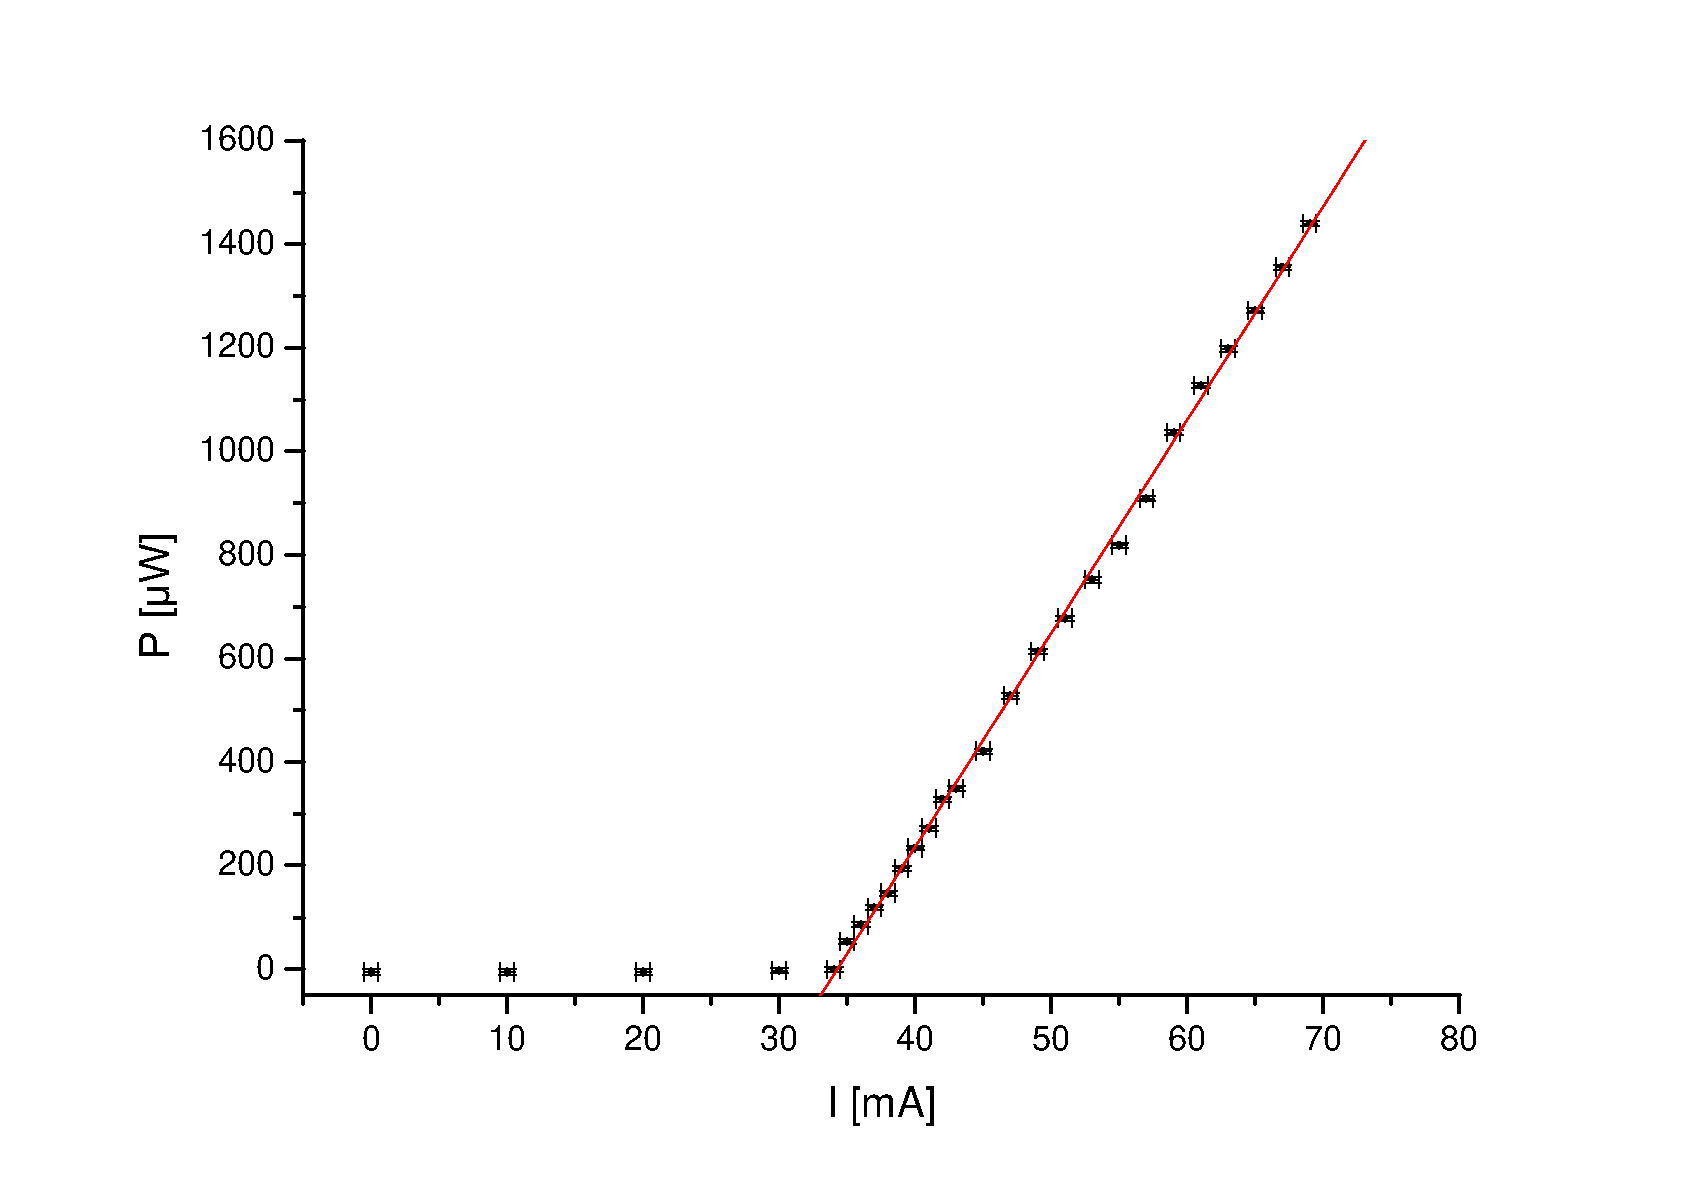
\includegraphics[width=0.6\textwidth]{graphics/Laserdiode_Plot}
	\caption{Plot der Messergebnisse zur Bestimmung der Kenngr��en der Laserdiode mit Fit an den Linearen Bereich}
	\label{fig:Laserdiode_Plot}
\end{figure}
\begin{table}[H]
  \centering
\resizebox{0.5\textwidth}{!}{
  \begin{tabular}{lc}
    \toprule
      &\\
    \midrule[0.75pt]
Schwellenstrom & $\unit{(34,26 \pm 0,01)}{\mathrm{mA}}$\\
differentieller Wirkungsgrad & $\unit{(41,218 \pm 0,009)}{\frac{\mu\mathrm{W}}{\mathrm{mA}}}$  \\
Quanteneffizienz & $26,422 \pm 0,006$\\
    \bottomrule
  \end{tabular}
}
 \caption{Zusammenfassung der Kenngr��en der Laserdiode}
  \label{tab:Laserdiode_Kenngroessen}
\end{table}
\section{Zusammenfassung}

\begin{appendix}

\section{Abbildungen}

\Literatur{quellen}

\end{appendix}
\end{document}


